\documentclass[aspectratio=169]{beamer}

% Paquetes necesarios
\usepackage[utf8]{inputenc}
\usepackage[spanish]{babel}
\usepackage{graphicx}
\usepackage{booktabs}
\usepackage{multirow}
\usepackage{colortbl}
\usepackage{adjustbox}
\usepackage{tikz}
\usepackage{makecell}

% =========================================================================
% DEFINICIÓN DE PALETA DE COLORES CORPORATIVA
% =========================================================================
\definecolor{DeepNavy}{HTML}{033b6d}
\definecolor{RoyalBlue}{HTML}{094b93}
\definecolor{OceanBlue}{HTML}{3077b9}
\definecolor{SkyBlue}{HTML}{a7d2f2}
\definecolor{SteelGrey}{HTML}{666766}

% =========================================================================
% CONFIGURACIÓN DEL TEMA BEAMER
% =========================================================================
\setbeamercolor{structure}{fg=DeepNavy}
\setbeamercolor{frametitle}{fg=DeepNavy, bg=SkyBlue!30}
\setbeamercolor{title}{fg=DeepNavy, bg=SkyBlue!20}
\setbeamercolor{item}{fg=RoyalBlue}
\setbeamercolor{block title}{bg=RoyalBlue, fg=white}
\setbeamercolor{block body}{bg=SkyBlue!10, fg=SteelGrey}

% Estilo de la fuente y de la barra de navegación
\setbeamertemplate{navigation symbols}{}
\setbeamertemplate{footline}[frame number]

% =========================================================================
% PORTADA
% =========================================================================
\title{\textbf{Resultados de la apliación}}
\subtitle{Prueba de Progreso Mes 4, 2026}
\author{Gerencia de Evaluación}
\date{Junio 2026}

\begin{document}

% -------------------------------------------------------------------------
% 1. SLIDE: TÍTULO
% -------------------------------------------------------------------------
\begin{frame}
    \titlepage
\end{frame}

% -------------------------------------------------------------------------
% SLIDE: COMPARATIVA MATEMÁTICA (MES 1 vs MES 2)
% -------------------------------------------------------------------------
\begin{frame}{Cobertura de Participación: Matemática y Lengua (Mes 4)}
    \vspace{-0.3cm}
    \begin{center}
    \adjustbox{max width=0.95\textwidth}{
        \renewcommand{\arraystretch}{1.3}
        \begin{tabular}{l c ccc ccc}
        \toprule
        \rowcolor{RoyalBlue}
        \textcolor{white}{\textbf{Grado}} & 
        \textcolor{white}{\textbf{Matrícula}} &
        \multicolumn{2}{c}{\textcolor{white}{\textbf{Matemática (MAT)}}} & 
        \multicolumn{2}{c}{\textcolor{white}{\textbf{Lengua (LEC)}}} \\
        \cmidrule(lr){3-4} \cmidrule(lr){5-6}
        \rowcolor{RoyalBlue}
        & \textcolor{white}{\textbf{Esperada}}
        & \textcolor{white}{\textbf{Participantes}} & \textcolor{white}{\textbf{\% Cobertura}}
        & \textcolor{white}{\textbf{Participantes}} & \textcolor{white}{\textbf{\% Cobertura}} \\
        \midrule
        2.$^\circ$ (Segundo)  & 14{,}265 &  9{,}309 & 65.3\% &  9{,}112 & 63.9\% \\
        3.$^\circ$ (Tercero)  & 14{,}766 &  9{,}726 & 65.9\% &  9{,}608 & 65.1\% \\
        4.$^\circ$ (Cuarto)   & 16{,}891 & 11{,}524 & 68.2\% & 11{,}448 & 67.8\% \\
        5.$^\circ$ (Quinto)   & 15{,}784 & 10{,}765 & 68.2\% & 10{,}729 & 68.0\% \\
        6.$^\circ$ (Sexto)    & 15{,}485 & 10{,}642 & 68.7\% & 10{,}602 & 68.5\% \\
        7.$^\circ$ (Séptimo)  & 16{,}081 & 10{,}799 & 67.2\% & 10{,}758 & 66.9\% \\
        8.$^\circ$ (Octavo)   & 15{,}460 & 10{,}517 & 68.0\% & 10{,}449 & 67.6\% \\
        9.$^\circ$ (Noveno)   & 13{,}992 &  9{,}541 & 68.2\% &  9{,}511 & 68.0\% \\
        10.$^\circ$ (1° Bach.) &  7{,}153 &  6{,}127 & 85.7\% &  6{,}089 & 85.1\% \\
        11.$^\circ$ (2° Bach.) &  6{,}034 &  5{,}333 & 88.4\% &  5{,}309 & 88.0\% \\
        \midrule
        \textbf{Total General} & \textbf{135{,}911} & \textbf{94{,}283} & \textbf{69.4\%} & \textbf{93{,}615} & \textbf{68.9\%} \\
        \bottomrule
        \end{tabular}
    }
    \end{center}
    \vfill
    \tiny \textcolor{SteelGrey}{\textit{Nota: Matrícula esperada según registro oficial. Solo población con pruebas válidas.}}
\end{frame}


% -------------------------------------------------------------------------
% SLIDE: BOXPLOTS B1 — MATEMÁTICA Y LENGUA (lado a lado)
% -------------------------------------------------------------------------
\begin{frame}{Distribución de puntajes para las escuelas del Bloque 1}
	\centering
	\begin{columns}[c]
		\begin{column}{0.5\textwidth}
			\centering
			
\includegraphics[width=\linewidth, height=0.88\textheight, keepaspectratio]{Graphs/Boxplot_Jitter_B1_Matemática.png}
		\end{column}
		\begin{column}{0.5\textwidth}
			\centering
			
\includegraphics[width=\linewidth, height=0.88\textheight, keepaspectratio]{Graphs/Boxplot_Jitter_B1_Lengua.png}
		\end{column}
	\end{columns}
\end{frame}

% -------------------------------------------------------------------------
% SLIDE: GRADOS 4°, 5°, 6° — LENGUA B1
% -------------------------------------------------------------------------
\begin{frame}{Niveles de Logro por Prueba --- Lengua B1 (4°, 5° y 6° Grado)}
    \centering
    \begin{columns}[c]
        \begin{column}{0.33\textwidth}
            \centering
            
\includegraphics[width=\linewidth]{Graphs/Barras_B1_Lengua_4_Grado.png}
        \end{column}
        \begin{column}{0.33\textwidth}
            \centering
            
\includegraphics[width=\linewidth]{Graphs/Barras_B1_Lengua_5_Grado.png}
        \end{column}
        \begin{column}{0.33\textwidth}
            \centering
            
\includegraphics[width=\linewidth]{Graphs/Barras_B1_Lengua_6_Grado.png}
        \end{column}
    \end{columns}
\end{frame}

% -------------------------------------------------------------------------
% SLIDE: GRADOS 7°, 8°, 9° — LENGUA B1
% -------------------------------------------------------------------------
\begin{frame}{Niveles de Logro por Prueba --- Lengua B1 (7°, 8° y 9° Grado)}
    \centering
    \begin{columns}[c]
        \begin{column}{0.33\textwidth}
            \centering
            
\includegraphics[width=\linewidth]{Graphs/Barras_B1_Lengua_7_Grado.png}
        \end{column}
        \begin{column}{0.33\textwidth}
            \centering
            
\includegraphics[width=\linewidth]{Graphs/Barras_B1_Lengua_8_Grado.png}
        \end{column}
        \begin{column}{0.33\textwidth}
            \centering
            
\includegraphics[width=\linewidth]{Graphs/Barras_B1_Lengua_9_Grado.png}
        \end{column}
    \end{columns}
\end{frame}

% -------------------------------------------------------------------------
% SLIDE: GRADOS 10°, 11° — LENGUA B1
% -------------------------------------------------------------------------
\begin{frame}{Niveles de Logro por Prueba --- Lengua B1 (10° y 11° Grado)}
    \centering
    \begin{columns}[c]
        \begin{column}{0.5\textwidth}
            \centering
            
\includegraphics[width=\linewidth]{Graphs/Barras_B1_Lengua_10_Grado.png}
        \end{column}
        \begin{column}{0.5\textwidth}
            \centering
            
\includegraphics[width=\linewidth]{Graphs/Barras_B1_Lengua_11_Grado.png}
        \end{column}
    \end{columns}
\end{frame}


% -------------------------------------------------------------------------
% SLIDE: GRADOS 2°, 3° — MATEMÁTICA B1
% -------------------------------------------------------------------------
\begin{frame}{Niveles de Logro por Prueba --- Matemática B1 (2° y 3° Grado)}
    \centering
    \begin{columns}[c]
        \begin{column}{0.5\textwidth}
            \centering
            
\includegraphics[width=\linewidth]{Graphs/Barras_B1_Matematica_2_Grado.png}
        \end{column}
        \begin{column}{0.5\textwidth}
            \centering
            
\includegraphics[width=\linewidth]{Graphs/Barras_B1_Matematica_3_Grado.png}
        \end{column}
    \end{columns}
\end{frame}

% -------------------------------------------------------------------------
% SLIDE: GRADOS 4°, 5°, 6° — MATEMÁTICA B1
% -------------------------------------------------------------------------
\begin{frame}{Niveles de Logro por Prueba --- Matemática B1 (4°, 5° y 6° Grado)}
    \centering
    \begin{columns}[c]
        \begin{column}{0.33\textwidth}
            \centering
            
\includegraphics[width=\linewidth]{Graphs/Barras_B1_Matematica_4_Grado.png}
        \end{column}
        \begin{column}{0.33\textwidth}
            \centering
            
\includegraphics[width=\linewidth]{Graphs/Barras_B1_Matematica_5_Grado.png}
        \end{column}
        \begin{column}{0.33\textwidth}
            \centering
            
\includegraphics[width=\linewidth]{Graphs/Barras_B1_Matematica_6_Grado.png}
        \end{column}
    \end{columns}
\end{frame}

% -------------------------------------------------------------------------
% SLIDE: GRADOS 7°, 8°, 9° — MATEMÁTICA B1
% -------------------------------------------------------------------------
\begin{frame}{Niveles de Logro por Prueba --- Matemática B1 (7°, 8° y 9° Grado)}
    \centering
    \begin{columns}[c]
        \begin{column}{0.33\textwidth}
            \centering
            
\includegraphics[width=\linewidth]{Graphs/Barras_B1_Matematica_7_Grado.png}
        \end{column}
        \begin{column}{0.33\textwidth}
            \centering
            
\includegraphics[width=\linewidth]{Graphs/Barras_B1_Matematica_8_Grado.png}
        \end{column}
        \begin{column}{0.33\textwidth}
            \centering
            
\includegraphics[width=\linewidth]{Graphs/Barras_B1_Matematica_9_Grado.png}
        \end{column}
    \end{columns}
\end{frame}

% -------------------------------------------------------------------------
% SLIDE: GRADOS 10°, 11° — MATEMÁTICA B1
% -------------------------------------------------------------------------
\begin{frame}{Niveles de Logro por Prueba --- Matemática B1 (10° y 11° Grado)}
    \centering
    \begin{columns}[c]
        \begin{column}{0.5\textwidth}
            \centering
            
\includegraphics[width=\linewidth]{Graphs/Barras_B1_Matematica_10_Grado.png}
        \end{column}
        \begin{column}{0.5\textwidth}
            \centering
            
\includegraphics[width=\linewidth]{Graphs/Barras_B1_Matematica_11_Grado.png}
        \end{column}
    \end{columns}
\end{frame}

% -------------------------------------------------------------------------
% SLIDE: BOXPLOT B2 — MATEMÁTICA Y LENGUA (lado a lado)
% -------------------------------------------------------------------------
\begin{frame}{Distribución por Prueba --- B2 (Todos los Grados)}
	\centering
	\begin{columns}[c]
		\begin{column}{0.5\textwidth}
			\centering
			
\includegraphics[width=\linewidth]{Graphs/Boxplot_Jitter_B2_Matemática.png}
		\end{column}
		\begin{column}{0.5\textwidth}
			\centering
			
\includegraphics[width=\linewidth]{Graphs/Boxplot_Jitter_B2_Lengua.png}
		\end{column}
	\end{columns}
\end{frame}

% -------------------------------------------------------------------------
% SLIDE: SANKEY B1 — TRAYECTORIAS MATEMÁTICA
% -------------------------------------------------------------------------
\begin{frame}{Trayectorias de Niveles --- B1 --- Matemática}
	\centering
	
\includegraphics[width=\textwidth]{Graphs/Sankey_Evolutivo_B1_Matemática.png}
\end{frame}

% -------------------------------------------------------------------------
% SLIDE: SANKEY B1 — TRAYECTORIAS LENGUA
% -------------------------------------------------------------------------
\begin{frame}{Trayectorias de Niveles --- B1 --- Lengua}
	\centering
	
\includegraphics[width=\textwidth]{Graphs/Sankey_Evolutivo_B1_Lengua.png}
\end{frame}

% -------------------------------------------------------------------------
% SLIDE: SANKEY B2 — TRAYECTORIAS MATEMÁTICA
% -------------------------------------------------------------------------
\begin{frame}{Trayectorias de Niveles --- B2 --- Matemática}
	\centering
	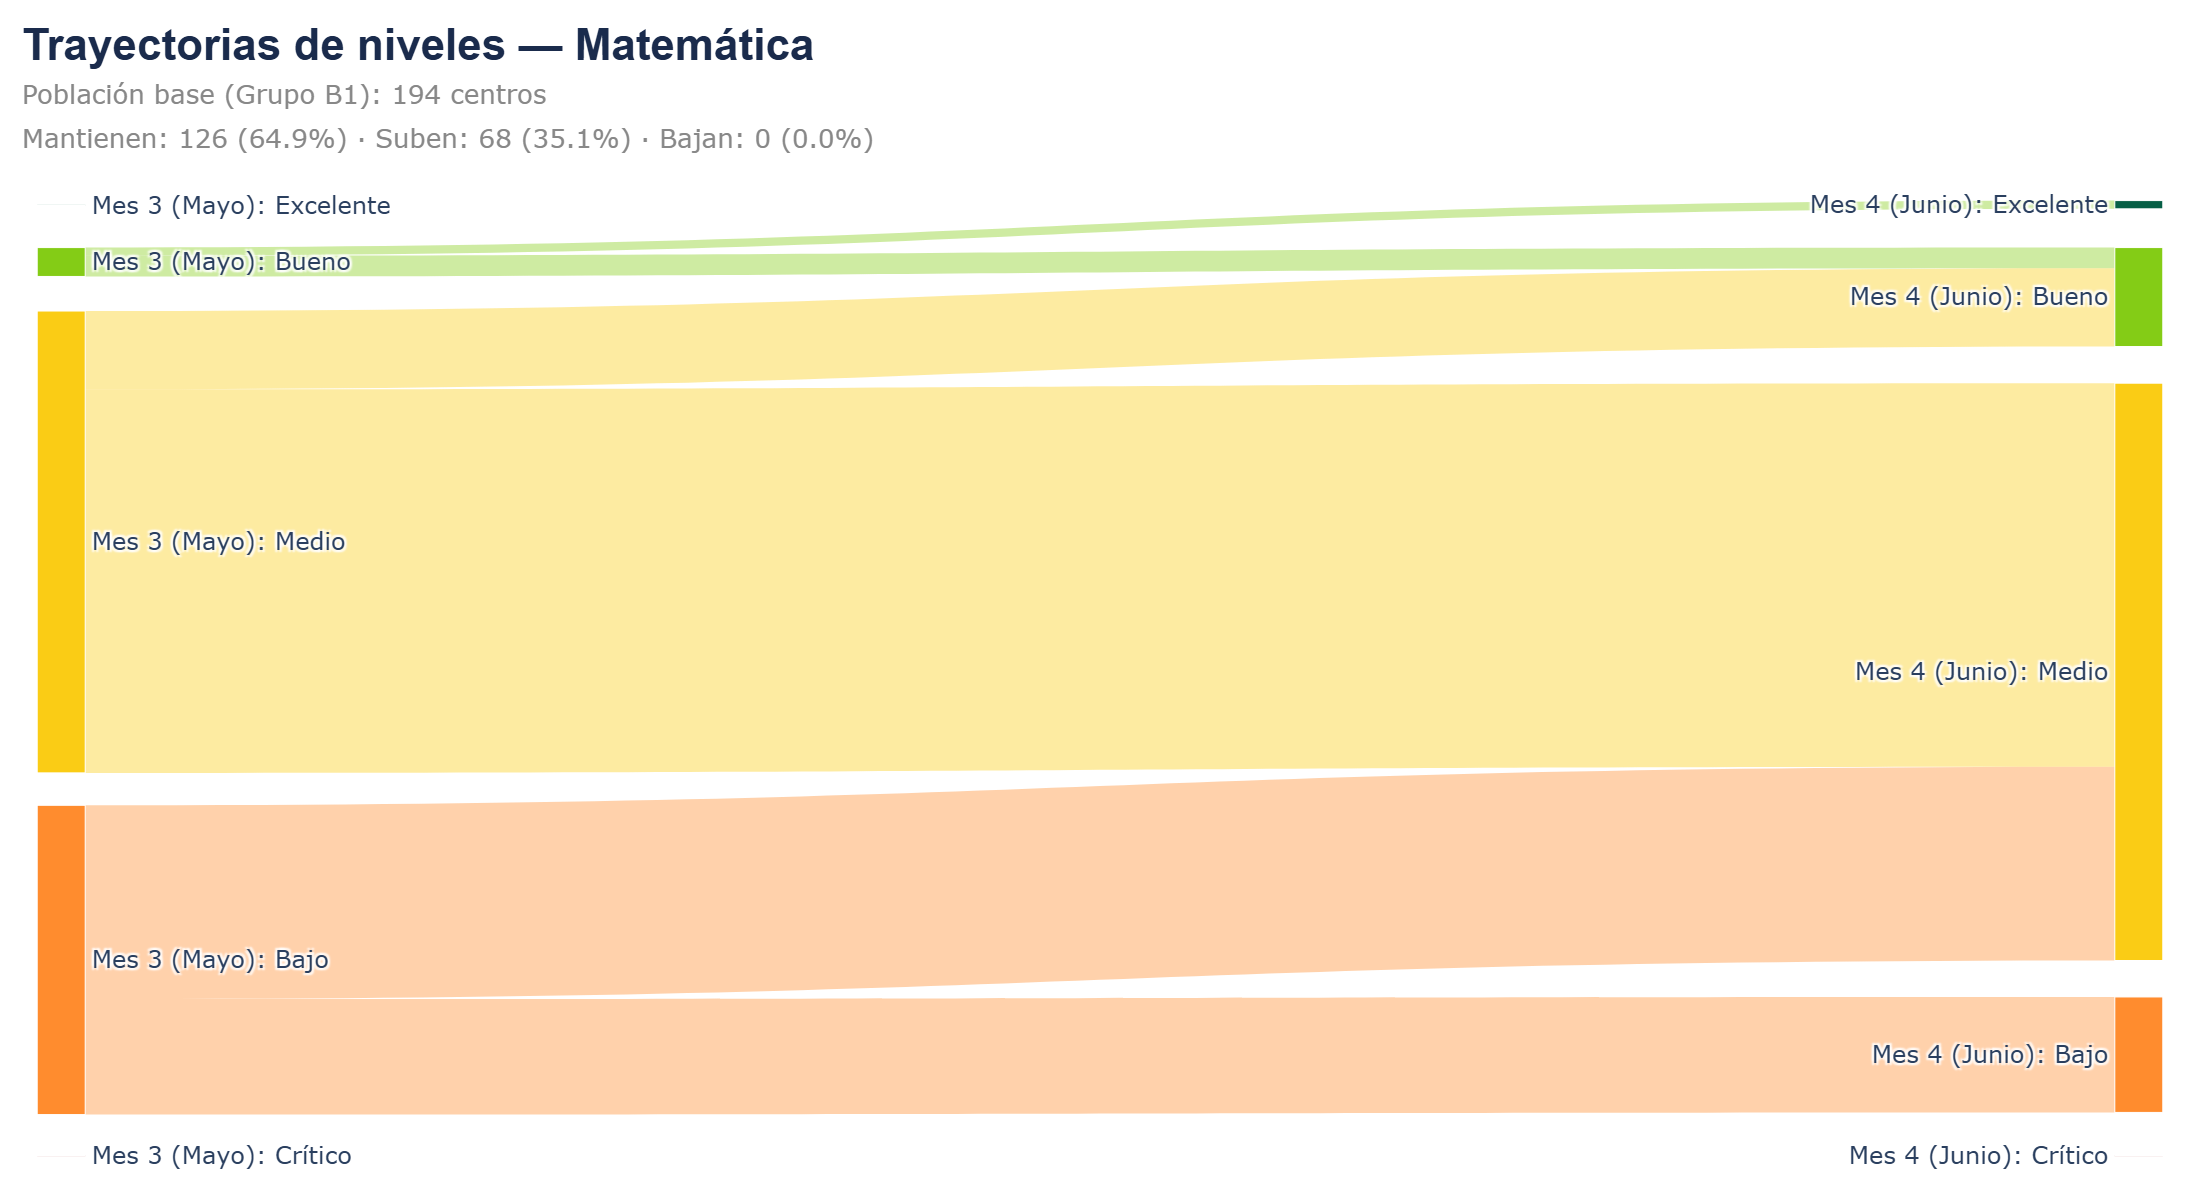
\includegraphics[width=\textwidth]{Graphs/Sankey_Evolutivo_B2_Matemática.png}
\end{frame}

% -------------------------------------------------------------------------
% SLIDE: SANKEY B2 — TRAYECTORIAS LENGUA
% -------------------------------------------------------------------------
\begin{frame}{Trayectorias de Niveles --- B2 --- Lengua}
	\centering
	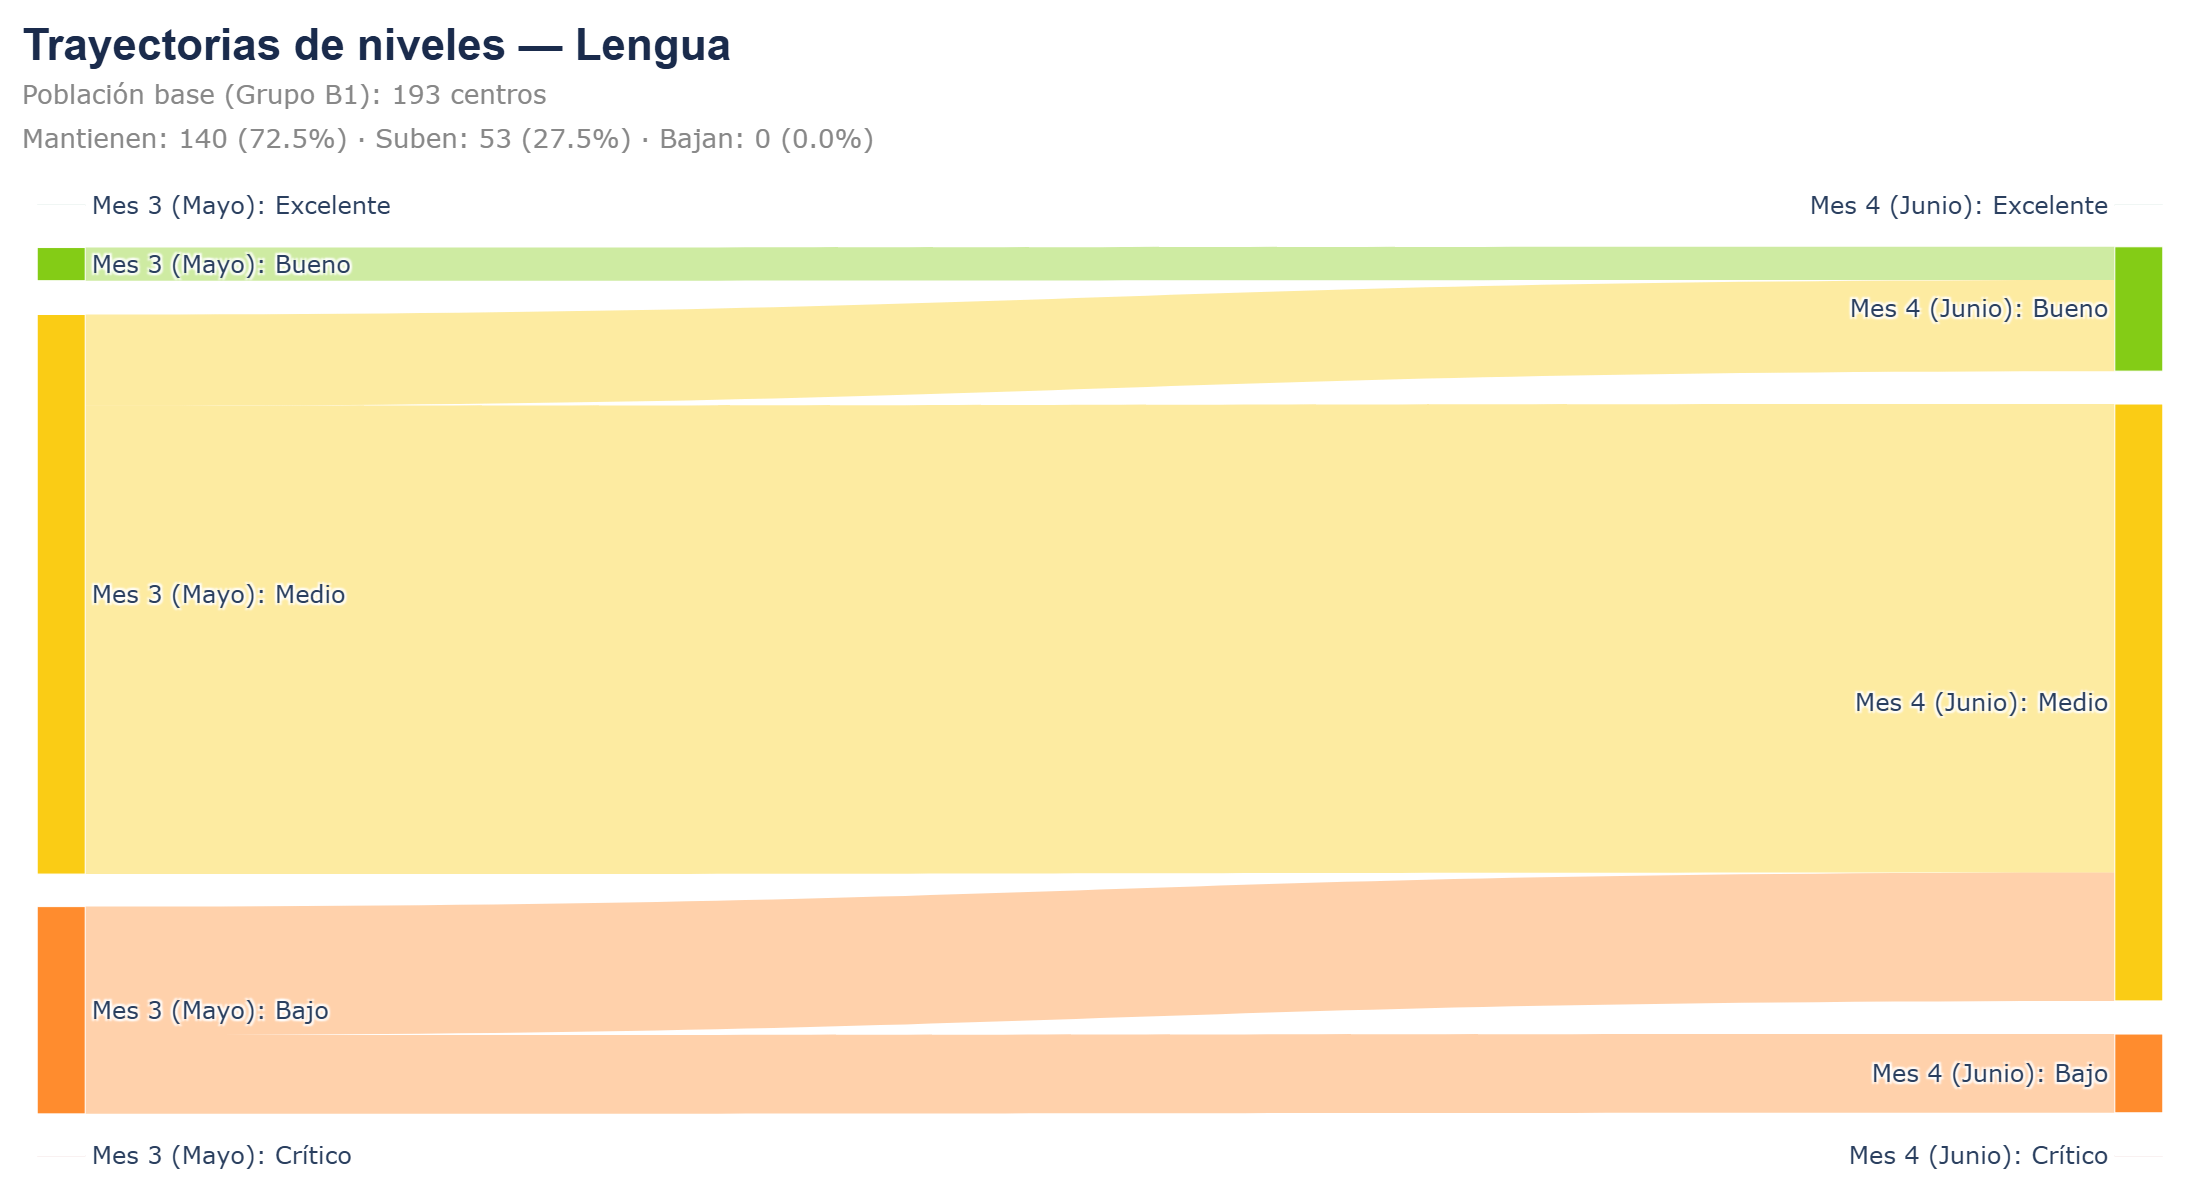
\includegraphics[width=\textwidth]{Graphs/Sankey_Evolutivo_B2_Lengua.png}
\end{frame}
\end{document}